\documentclass{article}

\usepackage{float}
\usepackage[utf8]{inputenc}
\usepackage[hidelinks, pdfauthor={Luc Gommans and Rick van Gorp}, pdftitle={TCP Congestion Algorithms in Datacenters}]{hyperref}
\usepackage[hyperref=true, natbib=true, style=numeric, backend=bibtex]{biblatex}
\usepackage{graphicx}
\bibliography{references.bib}
\usepackage[top=3.5cm, bottom=3.5cm, left=4.3cm, right=4.3cm]{geometry}


\setlength{\parindent}{0pt}
\setlength{\parskip}{\baselineskip}

\title{TCP Congestion Algorithms In Datacenters \\
	{\large Large Systems $\cdot$ Project Report}
}
\date{\today{}}
\author{Luc Gommans, Rick van Gorp}

\begin{document}
\maketitle

\section*{Abstract}

In datacenters, multiple tenants share a finite amount of bandwidth. When an
uplink is saturated, packets that overflow available buffer space will be
dropped and have to be retransmitted by the sender. When one tenant chooses to
retransmit faster than others, they have an advantage as they will make it
though more quickly. TCP is a connection-oriented protocol which employs
congestion control algorithms. These algorithms aim to divide the available
bandwidth equally between network flows.

Some congestion control algorithms are more aggressive than others, and it has
been reported that some algorithms cause others to back off excessively.
Tenants may, perhaps inadvertently, cause unequal bandwidth distributions during
times of congestion.

In this research, we compare five algorithms under different network conditions
to assess how they influence each other. We found that only CTCP (Windows)
backs off excessively; all other algorithms behave fairly. The results for CTCP
are anomalous compared to all other algorithms and we conclude that for this
algorithm, future work is needed for a reliable assessment.


\newpage
\section{Introduction}

Multitentant datacenters aim to provide services with consistent performance
and reliability. When customers send a lot of data in a short amount of time,
networks might become saturated or even congested, and bandwidth needs to be
distributed fairly among tenants.

Congestion occurs when a buffer on the path to the recipient is full and
packets have to be dropped. TCP uses a congestion control algorithm to avoid
congestion in the network and distribute bandwidth fairly among users. Several
algorithms are available to perform this function. Each has a different behaviour
depending on the network's characteristics.

This report includes a performance and behaviour analysis of different TCP
congestion control algorithms in a (simulated) multitenant datacenter network.
Mario Hock et al. describe in a paper that BBR shows unfair behaviour when
compared to the CUBIC congestion control
algorithm\cite{bbr-congestion-comparison}. Therefore the fairness between
congestion control algorithms will also be included in the analysis. Based on
the results, we will recommend datacenters on measures to take to keep
providing a reliable environment for customers when multiple congestion control
algorithms are active in the network, for example using Quality of Service or
prohibiting certain TCP congestion control algorithms. The main research question
is: {\it How can a datacenter provide a reliable and performing environment for
customers when multiple TCP congestion control algorithms are used in the
network?}

In the next section, we will discuss related work. Section \ref{sec:method}
describes our methods: how we selected algorithms to test, how we tested their
performance, and how we chose network conditions to simulate. Section
\ref{sec:results} describes the results of our research: the algorithms we
chose to test are described in \ref{sub:chosen-algos}, a theoretical analysis
of those is described in \ref{sub:algos-theoretical}, and experimental results
can be found in \ref{sub:experiment-results}. We discuss our results in section
\ref{sec:discussion}, mention possible future work in section
\ref{sec:futurework}, and finally draw conclusions in section \ref{sec:conclusion}.


\section{Related work}

In 2010, the algorithm DCTCP was described by Mohammad Alizadeh et
al.\cite{dctcp-congestion-original} and published as
RFC8257\cite{dctcp-congestion} in 2017. DCTCP is optimised for datacenters and
provides a high-burst tolerance, low latency, and high throughput when the
datacenter has a small part of the buffer available\cite{dctcp-congestion}.

In 2016 another algorithm was proposed: BBR. This is a TCP congestion algorithm
created by Google, which achieves higher bandwidths and lower latencies
compared to other TCP congestion methods\cite{bbr-congestion}. A comparison of
BBR with CUBIC\cite{bbr-congestion-comparison} shows that the BBR node pushes
the CUBIC node away in bandwidth when using small buffers. The BBR node gets
more bandwidth allocated than the CUBIC node.

The TCP congestion control algorithm BBR is discussed by Neal Cardwell et
al.\cite{bbr-congestion} The article contains a performance test of the BBR
algorithm and a comparison between the BBR algorithm and the CUBIC algorithm,
where a noticeable difference in bandwidth allocation is shown when using small
buffers.

A. Esterhuizen and A.E. Krzesinski\cite{multiple-congestion} analyse the
performance of multiple TCP congestion control algorithms, specifically: Reno,
BIC, CUBIC, HighSpeed TCP, TCP-Hybla, TCP-Illinois, TCP Low Priority,
TCP-Vegas, TCP-Westwood, TCP-YeAH, and Scalable TCP.


\section{Method}\label{sec:method}

During this research, performance comparison tests of various TCP congestion
control algorithms will be performed. The most common TCP congestion algorithms will be
determined through desk research. The tests will be conducted in an isolated
environment. Based on the results of those tests, recommendations will be given
related to the measures a datacenter has to take to keep the traffic equally
allocated over customers.


\subsection{Selecting TCP congestion algorithms}

In order to select the most common TCP congestion algorithms desk research will
be performed. This desk research will show which algorithms are used more often
than other algorithms by looking for the default algorithms in Operating
Systems. Based on those results, a list of TCP congestion algorithms will be
composed.


\subsection{Comparing Performance}

We will analyse one common scenario: multiple servers of different owners
inside a multitenant datacenter, sends data to clients outside the datacenter.
This could be users downloading software, the bursts while streaming a video
or movie, or large resources on a web page.

We will create a bottleneck on the path to the user to see how different
congestion control algorithms handle this. The connection will be full-duplex
and have symmetrical speeds, to avoid any congestion in sending
acknowledgements. Because the server is sending the large volume of data and
the client is responding with the much smaller acknowledgements, the server
will be the one applying congestion control. Therefore we vary the algorithm
settings of the server and not the client. The client will always be a
GNU/Linux machine using CUBIC, but we assume (due to the aforementioned
reasons) that this does not matter.

The bottleneck is created by having one receiving host, listening on different
ports, and two transmitting hosts. Each network interface is 1 gigabit per
second, thus the servers will have to limit their speed in order to avoid
flooding the client. This setup is shown in figure \ref{fig:setup1}.

We use three physical hosts as servers: two running Ubuntu 17.04 and one
running Microsoft Windows 10. In each experiment, only two hosts will be active.
The Windows system is used because there is no working CTCP
implementation---the default algorithm in Windows since Vista---available for a
modern Linux kernel.

\begin{figure}[H]
	\centering
		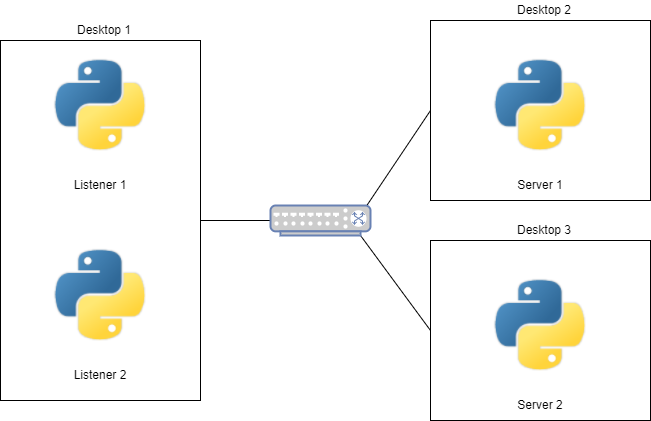
\includegraphics[scale=0.5]{figs/setup2.png}
		\caption{Test setup - Scenario 1}
	\label{fig:setup1}
\end{figure}

We will test the congestion algorithm for fairness in sharing bandwidth
with other TCP connections using other congestion algorithms. In order to test
the fairness, the bandwidth usage per second per algorithm is measured. If two
different algorithms use similar amounts of bandwidth, they can be said to be
fair relative to each other.

The tests conducted with the algorithms have two environment variables: packet loss and delay. Those environment variables are simulated using \texttt{netem}, which is a network emulation functionality in several Linux distributions\cite{linux-netem}. \texttt{netem} is applied to the incoming side of the interfaces of the clients to emulate the same packet loss and delay. Windows, which is tested as a server, does not support \texttt{netem}. Therefore the packet loss and delay are applied to the incoming interfaces of the clients. Packet loss and delay are chosen as the behaviour of most TCP algorithms depends on those variables\cite{bbr-congestion}\cite{dctcp-congestion}\cite{cubic-tcp-congestion}\cite{compound-tcp-congestion}\cite{bic-tcp-congestion}. The values for the environment variables are chosen based on measurements performed by Verizon\cite{verizon-latency}.

Each test is run at least twice. When results are conflicting or unexpected, we
ran a test more often and on different hardware.

%\item TCP Window Size measured over time: to determine whether using a specific TCP congestion algorithm in combination with other TCP congestion algorithms results in the allocation of a larger window or a smaller window to a specific TCP connection.
% \item Round Trip Time: to determine the reason of the behaviour of a TCP congestion algorithm in combination with other TCP congestion algorithms.


\subsubsection{Determining the Packet loss and Delay}

The data set of Verizon\cite{verizon-latency} is used to calculate the packet loss and delay used in this research. The data set includes global information and shows averages per month over the year 2017. The packet loss is calculated by taking the average of the Verizon Business Packet Delivery Statistics for Country Specific Metrics for each country. Those averages were inverted by subtracting the packet delivery percentage from 100, to show the actual packet loss in percentages and not the packet delivery. Based on the ascending sorted values a bar chart was created. This bar chart is shown in figure \ref{fig:packet-loss-chart}

\begin{figure}[H]
	\centering
		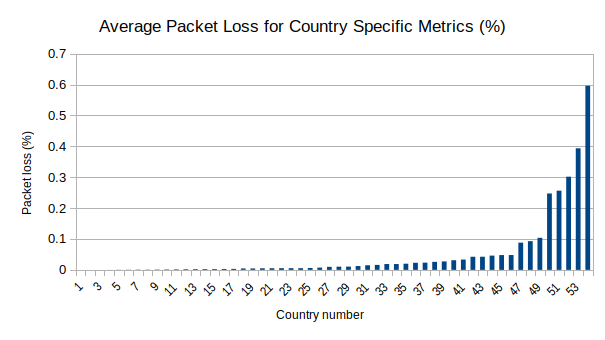
\includegraphics[scale=0.7]{figs/verizon-packetloss.png}
		\caption{Average Packet Loss for Country Specific Metrics}
	\label{fig:packet-loss-chart}
\end{figure}

The country numbers in figure \ref{fig:packet-loss-chart} are only used to show
the distribution of the average packet loss. The maximum average packet loss
shown in figure \ref{fig:packet-loss-chart} equals 0.6\% and the minimum equals
0\%. However, to account for situations where more packet loss occurs than usual,
the double value of the maximum is used: 1.2\%. The values for packet loss in
this comparison set-up were determined based on the distribution shown in
figure \ref{fig:packet-loss-chart} and the manually set maximum of 1.2\%. The
values are shown in table \ref{table:test-packetloss}.

\begin{table}[H]
	\centering
	\begin{tabular}[H]{ | l |}
	\hline
	\textbf{Packet loss} \\
	\hline 0\%. \\
	\hline 0.01\% \\
	\hline 0.1\% \\
	\hline 0.6\% \\
	\hline 1.2\% \\
	\hline
	\end{tabular}
	\caption{Packet loss percentages used for the comparison setup}
	\label{table:test-packetloss}
\end{table}

\vspace{0.9cm}

The delay is calculated by taking the average of the Verizon Business Latency
Statistics for Country Specific Metrics for each country. Based on the
ascending sorted values a bar chart was created. This chart is shown in figure
\ref{fig:verizon-delay-chart}.

\begin{figure}[H]
	\centering
		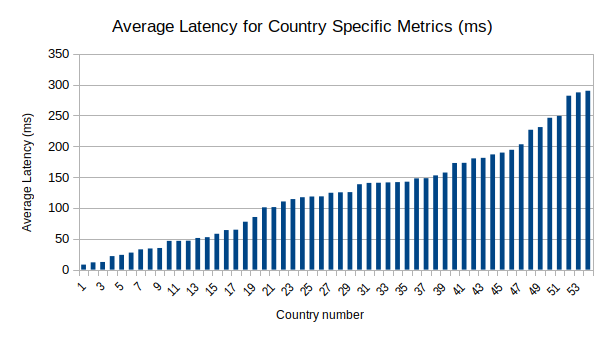
\includegraphics[scale=0.7]{figs/verizon-delay.png}
		\caption{Average Latency for Country Specific Metrics}
	\label{fig:verizon-delay-chart}
\end{figure}

The country numbers in figure \ref{fig:verizon-delay-chart} are only used to
show the distribution of the average delays. The maximum delay shown in figure
\ref{fig:verizon-delay-chart} equals 290ms and the minimum equals 8ms (both
rounded). The values for delay in this comparison set-up were determined based
on the distribution shown in figure \ref{fig:verizon-delay-chart}. The values
are shown in table \ref{table:test-delay}.

\begin{table}[H]
	\centering
	\begin{tabular}[H]{ | l |}
	\hline
	\textbf{Delay} \\
	\hline  8ms\\
	\hline  64ms  \\
	\hline  120ms  \\
	\hline  176ms \\
	\hline	232ms \\
	\hline  290ms  \\
	\hline
	\end{tabular}
	\caption{Packet loss percentages used for the comparison setup}
	\label{table:test-delay}
\end{table}


\subsubsection{Performing time-based automated tests}

The tests will be performed using scripts written in Python\cite{git-lsproj}.
All nodes run a client, which performs actions as instructed by the controller.
The controller is responsible for controlling the tests: synchronising time
among nodes, setting the TCP congestion algorithm of a node, and requesting one
node to open a listening port and instructing another to start sending at a
given time. Nodes report their measurements back to the controller.

\subsubsection{Testing hardware}

The specifications of the hardware used for the tests are shown in tables \ref{table:spec1} and \ref{table:spec2}.

\begin{table}[H]
	\centering
	\caption{Node configurations}
	\begin{tabular}[H]{ | l | l | }
	\hline
	\textbf{Hardware} & \textbf{Specification} \\
	\hline  Model & Dell Optiplex 7010\\
	\hline  CPU & Intel(R) Core(TM) i5-3570S CPU @ 3.10GHz\\
	\hline  Memory & 12GB\\
	\hline  NIC & Intel 82579LM Gigabit Network Connection (rev 04)\\
	\hline	NIC Driver & e100e 3.2.6-k\\
	\hline
	\end{tabular}
	\label{table:spec1}
\end{table}

\begin{table}[H]
	\centering
	\caption{Switch configuration}
	\begin{tabular}[H]{ | l | l | }
	\hline
	\textbf{Hardware} & \textbf{Specification} \\
	\hline  Model & 3Com OfficeConnect Gigabit Switch 16\\
	\hline  Ports & 16x Gigabit Ethernet\\
	\hline
	\end{tabular}
	\label{table:spec2}
\end{table}

\subsection{Traffic Management}

Desk research will be conducted to gather information related to traffic management. The goal is to find a mechanism that is capable of allocating bandwidth equally between customers of a datacenter. This is done by analysing the results from the algorithm comparison and the initial desk research on traffic management.


\section{Results}\label{sec:results}

In this section we will first elaborate on which algorithms we looked into, next we look at their internal workings, and finally we show the results of our experiments.


\subsection{TCP Congestion Algorithms}\label{sub:chosen-algos}

The most common TCP congestion algorithms are CTCP, CUBIC and BIC. CTCP is the default congestion algorithm in Microsoft Windows Server 2008 and newer\cite{cubic-kernel-version}. CUBIC is the default congestion algorithm in Linux distributions with kernel versions 2.6.19 and higher\cite{cubic-kernel-version}. BIC was the default congestion algorithm in earlier Linux distributions from kernel version 2.6.8 until 2.6.19\cite{bic-kernel-version}\cite{cubic-kernel-version}. DCTCP and BBR will also be tested as those protocols are new and upcoming---they are included in Linux since 4.9 (December 2016)\cite{linux-bbr}. DCTCP is specifically designed for datacenters\cite{dctcp-congestion} and BBR is a new algorithm meant for general use\cite{bbr-congestion}.


\subsection{Theoretical Algorithm Characteristics}\label{sub:algos-theoretical}

The BBR algorithm depends on parameters $BtlBw$ and $RT_{prop}$\cite{bbr-congestion}. Those parameters are estimates defined by the BBR algorithm. $BtlBw$ specifies the bandwidth at the slowest link in each direction and $RT_{prop}$ is the round-trip propagation time. $RT_{prop} = RTT - queuing delay - processing delay$, which results in the minimum amount of time for round trip propagation in case there are no queuing or processing delays. Using those two parameters, the Bandwidth Delay Product (BDP) is calculated, which is the maximum possible amount of data being sent in a network: $BDP = BtlBw * RT_{prop}$. As long as the amount of data in transit is less than the $BDP$ and $BtlBw$, the delivery rate is increased. If the amount of data in transit is equal to $BtlBw$ the delivery rate can not go up anymore. The $RTT$ can never be lower than $RT_{prop}$.

The CTCP algorithm is a combination of a loss-based and delay-based congestion protocol\cite{compound-tcp-congestion}. For the loss-based component, the variable conventional congestion window, $cwnd$, was introduced. For the delay-based component, the variable delay window, $dwnd$, was introduced. The TCP sending window is determined from: $win = min(cwnd + dwnd, awnd)$, where $awnd$ is the window advertised by the receiver. For $cwnd$ on the arrival of an ACK: $cwnd = cwnd + 1/win$. The $dwnd$ variable is initially set to zero and is only set when the congestion avoidance is active. $dwnd$ is calculated differently for several scenarios. If the network path is underutilised: $dwnd(t+1) = dwnd(t) + \alpha*dwnd(t)^{k} - 1$. When the network path is congested: $dwnd(t+1) = dwnd(t) - \eta*diff$. When packet loss occurs: $dwnd(t+1) = dwnd(t)(1-\beta) - cwnd/2$. $k$, $\alpha$, $\eta$ and $\beta$ are tunable parameters for optimisation of the algorithm. $\eta$ defines the rapidness of reduction of the window when congestion is detected. $\beta$ is the factor used for the multiplicative decrease after loss is detected. $diff$ is calculated from the expected throughput and the actual throughput, which are again calculated from the window size and Round Trip Time (RTT).

The DCTCP algorithm\cite{dctcp-congestion-original} consists of three components:

\begin{enumerate}
	\item Simple Marking at the Switch. Based on the marking threshold $K$ a packet is marked with the CE flag. This only occurs when the queue occupancy is greater than K at arrival time. The marking threshold $K$ specifies the minimum value of queue occupancy.
	\item ECN-Echo at receiver. The receiver running the DCTCP algorithm ACKs every packet and sets the ECN-Echo flag only if the packet was marked with CE. The ECN-Echo flag is used to notify the sender of congestion in the network.
	\item Controller at the sender. The sender has an estimate of the fraction of packets that are marked with CE. This is based on the actual fraction of packets that were marked, the weight given to the new estimate compared to the past weight. This results in $\alpha$. $\alpha$ is used to indicate the congestion on a network with a maximum of value 1, indicating a congested network, and a minimum value of 0, indicating no congestion in the network. DCTCP cuts the window size using $\alpha$: $cwnd = cwnd * (1 - \alpha/2)$. This results in a low queue length, but ensuring high throughput.\\
\end{enumerate}

The BIC algorithm controls its windows based on the size of windows\cite{bic-tcp-congestion}. It consists of two components:

\begin{enumerate}
	\item Binary search increase. This algorithm computes the midpoint between the maximum window size $W_{max}$ and current minimum window size $W_{min}$. If packet loss occurs, $W_{max}$ is set to the midpoint. This process repeats until $W_{max}$ and $W_{min}$ are smaller than the minimum increment $S_{min}$.
	\item Additive increase runs as an addition to the binary search increase. If $W_{max} - midpoint > S_{max}$, the window size is increased by $S_{max}$ until $W_{max} - midpoint < S_{max}$. $S_{max}$ is the preset maximum increment.
\end{enumerate}
In case the current window size becomes greater than $W_{max}$ a slow start strategy is performed to determine a new $W_{max}$: $W_{max} + \alpha * S_{min}$, where $\alpha$ is a multiplier. The multiplier is increased by one until $S_{min} * \alpha >= S_{max}$ or when losses occur. In the case of loss a new value for $W_{max}$ will be set.

The CUBIC algorithm is a successor of the BIC algorithm\cite{cubic-tcp-congestion}. In case of a loss event $W_{max}$, which is the maximum window size, is registered. This is followed by a multiplicative decrease of the congestion window by factor $\beta$. If an ACK in congestion avoidance is received and the current window size $cwnd$ is less than $W_{max}$, the algorithm uses the concave profile to increase the window size according to the formula: $cwnd = \frac{W(t+RTT)-cwnd}{cwnd}$. If $cwnd$ is larger than $W_{max}$, the convex profile is used to increase the window size according to the same formula as the concave profile. In both formulas $t$ is the time elapsed from the last window reduction.


\subsection{Experiments' Results}\label{sub:experiment-results}

In our results, we see that all algorithms clearly respond to the simulated
network circumstances, but not very much to each other. Most algorithms are
fair towards all other algorithms and will use their half of the connection.
See figures \ref{fig:fair-1} and \ref{fig:fair-2}. In figure \ref{fig:fair-1} we see that in the first test run, the increase of BIC is more aggressive than CUBIC's. This is related to the difference in increase functions used by both TCP congestion algorithms. In figure \ref{fig:fair-2} we also see that the increase of BIC is more aggressive than DCTCP's. BIC's increase function is characterised to be more aggressive and that can be seen in the graph as the increase line is more steep. The differences in those increase functions, however, do not show any implications on the fairness of the algorithms as the bandwidth allocation is near to equal for both algorithms. 

\begin{figure}[H]
	\makebox[\textwidth]{
		\centering
		\begin{minipage}{0.5\paperwidth}
			\centering
			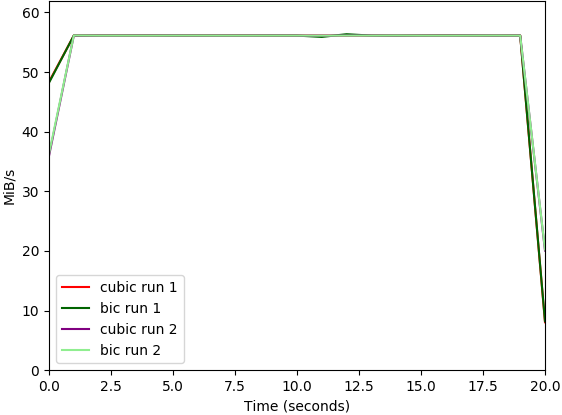
\includegraphics[width=0.9\textwidth]{figs/cubic_vs_bic_8_0.png}
			\caption{CUBIC vs. BIC with 8ms latency and 0\% loss}
			\label{fig:fair-1}
		\end{minipage}\hfill
		\begin{minipage}{0.5\paperwidth}
			\centering
			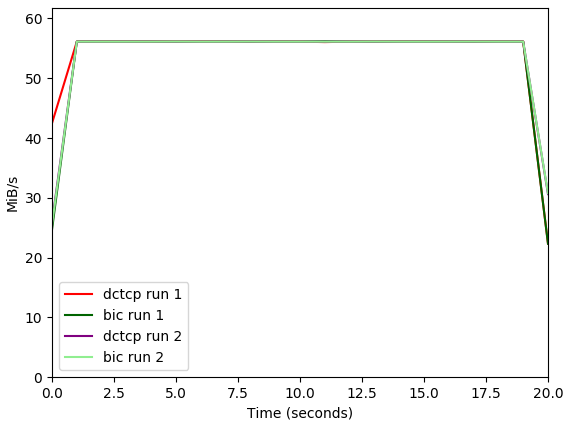
\includegraphics[width=0.9\textwidth]{figs/dctcp-bic-8-0.png}
			\caption{DCTCP vs. BIC with 8ms latency and 0\% loss}
			\label{fig:fair-2}
		\end{minipage}
	}
\end{figure}

CTCP is the only algorithm that responds excessively to others. Alone, it
reaches the full gigabit speed; but if any other algorithm runs at the same
time (i.e. a normal test is performed), CTCP's speed consistently drops. It
then reaches around 57 megabits ($\pm$6.8MiB/s), while the other algorithms reach at
least 800 with good network conditions (8 milliseconds latency, 0\% loss).
See figure \ref{fig:ctcp-1} for an example of BIC vs. CTCP.

\begin{figure}[H]
	\centering
		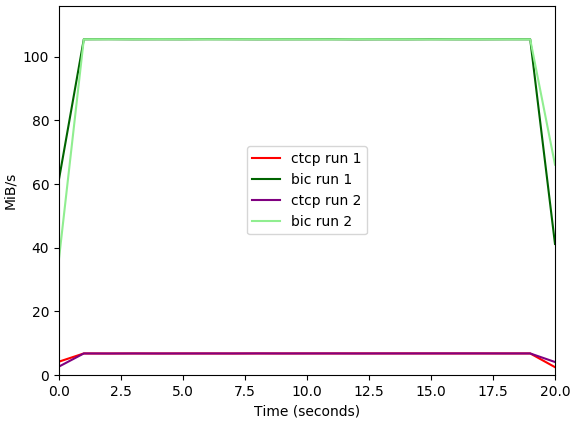
\includegraphics[scale=0.55]{figs/ctcp-bic-8-0.png}
		\caption{CTCP vs. BIC with 8ms latency and 0\% loss}
	\label{fig:ctcp-1}
\end{figure}

Additionally, CTCP also lowers its speed in response to the simulated network
circumstances: with 1.2\% packet loss and 8 milliseconds latency, it will reach
around 25 megabits, and with 290 milliseconds latency and no loss, it reaches
around 1.5 megabits. In neither case does it reach the original 55 megabits.

Because of the exceptional results for CTCP, we performed the test again on
different hardware. This yielded the same result. To verify that it is CTCP and
not our software that performs differently on Windows, we setup a small
experiment using \texttt{iperf}. The setup was the same as our original
experimental setup with one sender on two hosts and two receivers on one host,
only we manually started \texttt{iperf} bandwidth tests rather than doing it in
an automated fashion with Python. In this instance, Windows performed normally
and did not back off exceptionally when introducing another contender.

%\newgeometry{top=1cm,bottom=1.5cm}

BBR is unique in that it barely responds to packet loss but only to delay: even
with 1.2\% loss, as long as the delay is low (8 milliseconds in our case), it
reaches 850$\pm$20 megabits per second. A comparison between BBR and CUBIC is shown in figure \ref{fig:bbr-cubic}. We see in figure \ref{fig:bbr-cubic} that, compared to CUBIC, the bandwidth usage by the BBR data transfer is higher when 1.2\% packet loss is introduced. However, the link speed of 1Gbps is not fully utilized as is in the paper written by Mario Hock et al.\cite{bbr-congestion-comparison}. We also do not see the CUBIC data transfer responding to the BBR data transfer by reducing its speed in any way. In another test, where CUBIC is compared to BIC with the same parameters, we see CUBIC utilizing the same amount of bandwidth as in the BBR-CUBIC comparison. This is shown in figure \ref{fig:bic-cubic}. In figure \ref{fig:bbr-cubic-0} we show a comparison of a CUBIC data transfer with a BBR data transfer with parameters 8ms latency and 0\% packet loss. This time the total link speed is utilized and we see no unfairness between CUBIC and BBR. We therefore see no signs in our results of BBR being the cause of the CUBIC data transfer being slower. In our results other algorithms also reach much lower
speeds (24 megabits is not uncommon), but we see no signs of BBR being the
cause of that. In tests with BBR nor CTCP, speeds are not higher than when BBR
is one of the algorithms being tested.

\begin{figure}[H]
	\makebox[\textwidth]{
		\centering
		\begin{minipage}{0.5\paperwidth}
			\centering
			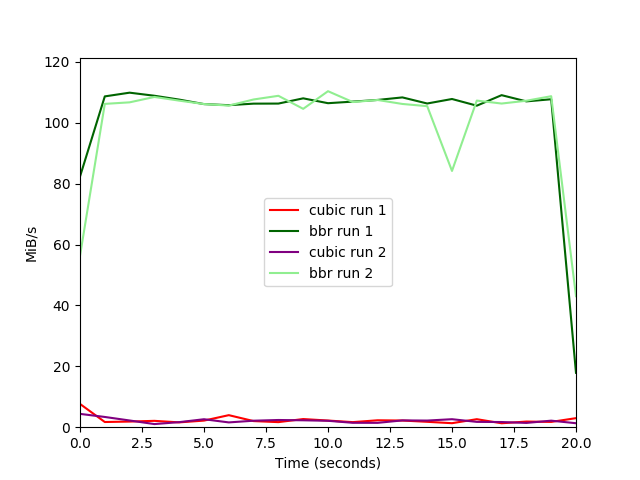
\includegraphics[width=0.9\textwidth]{figs/cubic_vs_bbr_8_12.png}
			\caption{CUBIC vs. BBR with 8ms latency and 1.2\% loss}
			\label{fig:bbr-cubic}
		\end{minipage}\hfill
		\begin{minipage}{0.5\paperwidth}
			\centering
			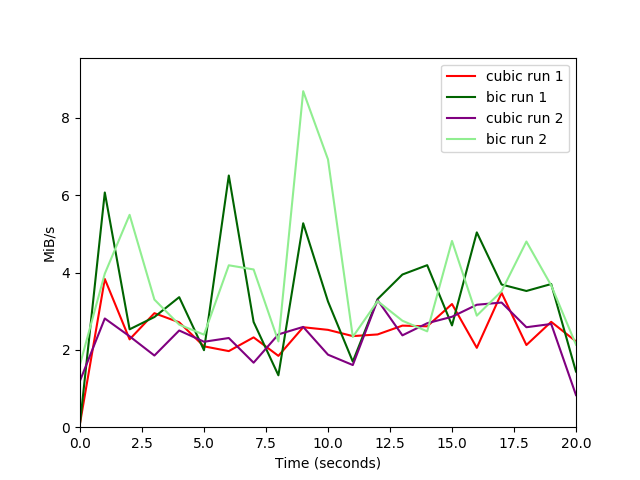
\includegraphics[width=0.9\textwidth]{figs/cubic_vs_bic_8_12.png}
			\caption{CUBIC vs. BIC with 8ms latency and 1.2\% loss}
			\label{fig:bic-cubic}
		\end{minipage}
	}
\end{figure}

\begin{figure}[H]
	\centering
		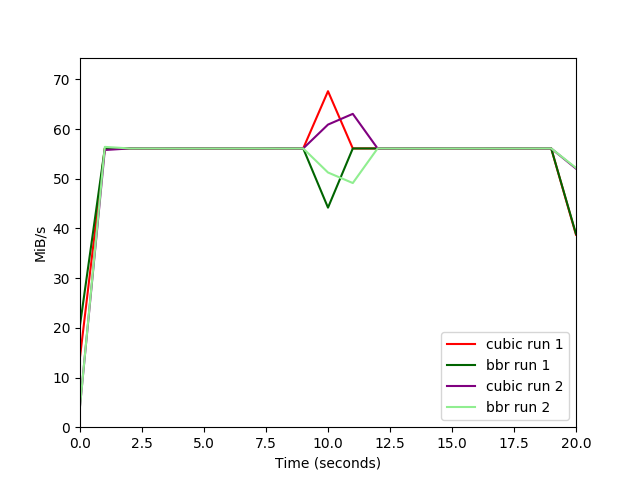
\includegraphics[scale=0.6]{figs/cubic_vs_bbr_8_0.png}
		\caption{CUBIC vs. BBR with 8ms latency and 0\% loss}
	\label{fig:bbr-cubic-0}
\end{figure}

The full set of results is available online\cite{git-lsproj}.

%\restoregeometry


\subsection{Traffic Management}

Our results show that traffic management is currently not necessary. However, a
tenant might purposefully install an unfair algorithm. In this section we
discuss different possible approaches a datacenter could take.

We propose two possible solutions to manage traffic from a multitenant
datacenter to customers when unfair TCP congestion control algorithms are used:
traffic shaping based monitoring, and detection of unaccepted TCP congestion
algorithms in the network. 

\subsubsection{Traffic shaping based Monitoring}

With the use of a hypothetical congestion control algorithm which is unfair towards other flows, the bandwidth allocation to one customer would be higher than to other customers. When a TCP flow shows an aggressive increase and keeps pushing data over the network, other (fair) algorithms will reduce the transmission rate as packet loss occurs. One important condition for this unfair congestion control algorithm is that it should not be aggressive to the extent of causing a denial of service.

To mitigate this, the bandwidth usage per server could be monitored, prioritising the traffic sent by some servers. The monitor uses traffic shaping to control the priority of the traffic per server:

\begin{enumerate}
	\item The monitor measures periodically whether the bandwidth in the link is fully utilised. If this is the case, the next step will be performed. If not, it continues monitoring the link utilisation.
	\item The monitor calculates periodically, per server, whether its bandwidth usage deviates more than $\alpha$ from the average bandwidth usage. $\alpha$ is the deviated bandwidth and is set according to an acceptable deviation value. The following formula is used to calculate the standard deviation: $s_{i} = \sqrt{\frac{\sum_{i=1}^N (x_i - \overline{x})^2}{N-1} }$. $N$ is the amount of active servers on the link. $\overline{x}$ is the average amount of bandwidth for all active servers on the link. $x_i$ is the bandwidth of the current server and $s_{i}$ shows the standard deviation in bandwidth for server $i$. If $s_{i}$ is a negative value, no priority change will be applied as the bandwidth usage is lower than average for the server. If $s_{i} <= \alpha$, then no priority change will be applied. If $s_{i} > \alpha$, the priority will be changed to a lower value.
	\item The monitor provides information of the servers where the priority will be set to a lower value to the traffic shaping controller.
	\item The traffic shaping controller sets the priority for the servers to a lower value, so that the traffic coming from the servers that use $\alpha$ more than average bandwidth has less preference than traffic closer to the average bandwidth and lower.
	\item The monitor periodically checks if the bandwidth in the link is still fully utilised. If this is not the case, the traffic shaping policy is reversed again by setting the priority to the default value. If this is the case, the periodical calculations of server bandwidth usage are continued.
\end{enumerate}

\subsubsection{Detection of unaccepted TCP congestion control algorithms}

Peng Yang et al.\cite{tcp-congestion-identification} describe a method to
remotely identify used TCP congestion avoidance algorithms. The paper states
that they were able to identify all default TCP algorithms, but some
non-default algorithms could not be identified. The tests performed are limited
to remote web servers, so it requires adaption to implement such a method in a
generic manner. If this method is deemed reliable, it can be useful to detect
whether an unfair algorithm is used as it will not match
any of the default algorithms used. Based on that, the traffic of the
unacceptable TCP congestion control algorithms can be shaped by lowering their
priority.


\section{Discussion}\label{sec:discussion}

The CTCP measurements were done on a Windows 10 machine because there is no
up-to-date implementation of CTCP for Linux. All other measurements were done
on machines running Ubuntu 17.04. This might have introduced issues while
measuring the CTCP algorithm versus any other congestion algorithm. According
to our measurements, all other algorithms are fair in sharing bandwidth with
each other; only CTCP consistently and excessively reduced its bandwidth
allocation.

Without any concurrent flows, Windows does reach the full link speed (1Gbps).
On different hardware, it showed the same, recessive behaviour. We
think this might be caused by the way Python socket operations are handled in
Windows. When repeating the test with \texttt{iperf}, which is written in C,
this behaviour no longer occurs. Even when using the Python equivalent of
\texttt{while(true)\{ socket.send(data); \}}, the bandwidth allocation did not
change. We theorise that the difference is caused by something in the
\texttt{send} call. An alternative theory is that Microsoft Windows for
workstations have a different implementation than Microsoft Windows Server
systems.

BBR is the best-performing algorithm in our set, because it barely responds to
packet loss. However, we were unable to draw the same conclusions to our
results as the conclusions written in the paper by Mario Hock et
al\cite{bbr-congestion-comparison}. We used multiple values to simulate packet
loss as well as delay, which simulate having small buffers. BBR is a TCP
congestion control protocol that reacts to the minimum RTT in combination with
the Bottleneck Bandwidth. We have tested multiple delay values that appear in
the real world. The delay values are directly related to the minimum RTT
possible on the link. As mentioned in the results, we see no hard evidence that
this causes other algorithms to reduce their speed further, but there are
slight indications. For example in the test of DCTCP versus BBR, DCTCP reaches
around 0.2 to 0.6 megabytes per second. In the test of DCTCP versus BIC, this
is 0.3 to 0.7 megabytes per second. The difference is large nor statistically
significant, but it warrants looking into. On the scale of 0.7 megabytes per
second, a tenth of a megabyte does make a difference.


\section{Future work}\label{sec:futurework}

Running a mixed environment of Linux and Windows introduced issues, at least in
combination with Python as benchmark system. We expect that in Windows, the
Python send call on sockets is implemented differently than in Linux, but this
requires more testing. The tests for CTCP should be performed again when the
reason for the discrepancy is known and can be mitigated. The results should
also be verified using a Microsoft Windows Server instance.

Our tests were done using three nodes in a switched network. To make sure our
results hold in practice, future work could introduce a routed network with
many more nodes.

In this paper we have proposed a monitoring solution, which checks for the deviation between the server bandwidth on a link and the average bandwidth used by servers on a link. This solution requires performance testing, such that it is capable of running in a datacenter and not causing delay. Also an $\alpha$ value has to be determined that works in most environments, without ruling out servers that are not running unfair TCP congestion protocols.

BBR performs better in a congested network than any other tested algorithm.
While we did not see clear signs of other algorithms responding to BBR's higher
bandwidth share, this should be tested further to be certain. We suggest
starting a transfer with one algorithm under the desired network circumstances,
determine its bandwidth, and then start a parallel flow using BBR. If the
bandwidth of the original flow does not decrease, BBR is indeed fair towards
this algorithm.


\section{Conclusion}\label{sec:conclusion}

Our main research question is: {\it How can a datacenter provide a reliable and performing environment for customers when multiple TCP congestion control algorithms are used in the network?} 

For the algorithms BIC, BBR, CUBIC and DCTCP, we conclude that, based on the setup we have used, they allocate
bandwidth fairly and do not suppress each other. There is no impact on the
service for customers when using those algorithms mixed in one environment.

CTCP, the default algorithm for Microsoft Windows, shows inconclusive results
and we can not draw any conclusions with regards to this algorithm.

In our results, BBR shows better performance than any other algorithm when
packet loss occurs. Finally, DCTCP is only suitable when both the server and
client are in the same datacenter: there is a considerable ramp-up time when
congestion occurs. Within datacenters DCTCP works well, because without
congestion it keeps queue lengths to a minimum.

\printbibliography

\end{document}

